\subsubsection{Database design}
	What follows is the class diagram representation of the database designed to store the data needed by the system. It embodies the data layer, and is stored by \textit{database servers}, which also provides access to it.\newline
	The reader will find comments on the diagram itself: they mainly reflect some constraint on the data represented, and are connected directly to the elements involved.\newline

	\begin{sidewaysfigure}
		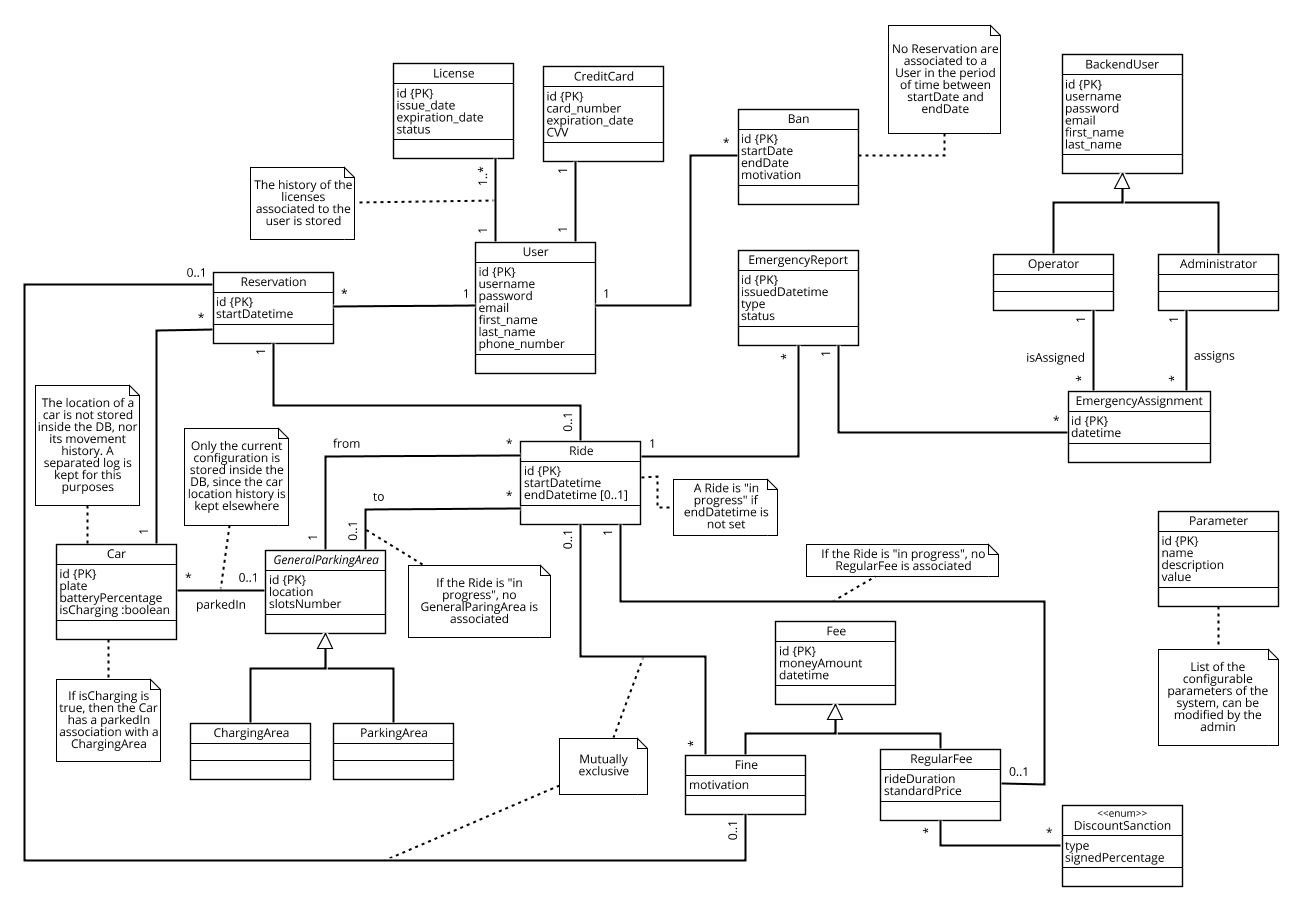
\includegraphics[width=\hsize, center]{img/db_class_diagram.png}
		\caption{Database design.}
	\end{sidewaysfigure}

	\noindent A clarification is needed, although a comment already summarizes it. The database stores the current state of the system as well as the history of its changes. The only exception to this policy is represented by the car location: given the high level of changes in the position of the car, due to its role in the system, it would be inefficient and resource-consuming to store all this information in a relational database. For this reason, a specific log - here not analysed - is introduced to keep track of the car movements and be able to retrieve them when needed (i.e. legal matters, theft, etc.).
\FloatBarrier
